


\chapter{Podstawy teoretyczne estymacji parametrów wydolnościowych z wykorzystaniem uczenia maszynowego}

Wydolność tlenowa w kolarstwie jest jednym z kluczowych czynników determinujących wynik sportowy \cite{borszcz2018ftp}.
Jej ilościowy opis od lat stanowi przedmiot badań fizjologów wysiłku i trenerów.
W praktyce treningowej potrzebne są wskaźniki, które z jednej strony dobrze odzwierciedlają możliwości zawodnika, a z drugiej są możliwe do regularnego monitorowania w warunkach terenowych.
Jednym z najczęściej stosowanych parametrów jest funkcjonalny próg mocy (ang. \textit{Functional Threshold Power}, $\mathrm{FTP}$) \cite{borszcz2018ftp,allen2019power}.

Rozwój czujników pomiaru mocy, opasek rejestrujących tętno oraz szerokie wykorzystanie liczników rowerowych i platform treningowych powoduje, że powstają liczne zbiory danych treningowych.
Dane te mogą zostać wykorzystane w modelach uczenia maszynowego do estymacji $\mathrm{FTP}$ na podstawie codziennych jazd, bez potrzeby wykonywania osobnych, wyczerpujących testów.

W niniejszym rozdziale przedstawiono podstawowe pojęcia związane z $\mathrm{FTP}$, charakterystykę danych wykorzystywanych w dalszej części pracy oraz przegląd wybranych metod szacowania parametrów wydolnościowych z użyciem klasycznych podejść i uczenia maszynowego.

\section{FTP jako parametr wydolności}

Funkcjonalny próg mocy ($\mathrm{FTP}$) jest jednym z najczęściej stosowanych w praktyce treningowej wskaźników wydolności tlenowej kolarzy \cite{borszcz2018ftp,allen2019power}.
Intuicyjnie można go opisać jako „moc, którą kolarz jest w stanie utrzymać przez dłuższy czas bez narastającego, gwałtownego zmęczenia”.
W przeciwieństwie do prostych wartości maksymalnych (np.\ maksymalnej mocy szczytowej czy tętna maksymalnego), $\mathrm{FTP}$ odnosi się do zdolności organizmu do długotrwałego utrzymania wysokiej, ale jeszcze zrównoważonej intensywności wysiłku.
Z tego powodu parametr ten dobrze nadaje się do opisu poziomu sportowego i planowania treningu wytrzymałościowego.

\subsection{Definicja funkcjonalnego progu mocy}

W literaturze związanej z treningiem kolarskim parametr $\mathrm{FTP}$ najczęściej definiuje się jako najwyższą wartość mocy, jaką kolarz jest w stanie utrzymać w stanie quasi-stacjonarnym przez około $60$ minut \cite{borszcz2018ftp,allen2019power}.
„Quasi-stacjonarny” oznacza tutaj, że reakcja fizjologiczna organizmu (w szczególności tętno, wentylacja oraz stężenie mleczanu we krwi) stabilizują się na podwyższonym, ale względnie stałym poziomie.
W praktyce przyjmuje się, że przy mocy równej $\mathrm{FTP}$ parametry te nie narastają już gwałtownie, natomiast przekroczenie tej intensywności prowadzi do szybkiego narastania zmęczenia i konieczności zredukowania mocy \cite{borszcz2018ftp,karsten2021cpftp}.

Ze względów praktycznych $\mathrm{FTP}$ rzadko wyznacza się z pełnego, $60$-minutowego testu czasowego.
Taki test jest bardzo obciążający, wymaga odpowiednich warunków i trudno go często powtarzać.
Dlatego w treningu amatorskim i zawodowym spopularyzowały się krótsze protokoły, z których najpopularniejszy jest $20$-minutowy test maksymalny \cite{allen2019power}.
Uproszczona wersja polega na wykonaniu rozgrzewki, a następnie jeździe z maksymalnym możliwym wysiłkiem  przez $20$ minut.
Średnia moc z tego odcinka jest następnie mnożona przez współczynnik (najczęściej $0{,}95$), co ma przybliżać moc, jaką kolarz byłby w stanie utrzymać przez $60$ minut \cite{allen2019power,sitko2023update}.

\begin{equation}
\label{eq:ftp_20min}
\mathrm{FTP} \approx 0{,}95 \cdot \overline{P}_{20\ \mathrm{min}},
\end{equation}
gdzie $\overline{P}_{20\ \mathrm{min}}$ oznacza średnią moc w $20$-minutowym odcinku testowym.

Warto podkreślić, że jest to definicja funkcjonalna, a nie „fizjologiczna” w ścisłym sensie.
$\mathrm{FTP}$ nie jest bezpośrednim pomiarem żadnego pojedynczego mechanizmu w organizmie (np.\ maksymalnego poboru tlenu), lecz wygodnym parametrem łączącym w sobie kilka aspektów wydolności: zdolność do generowania mocy, tolerancję zmęczenia i efektywność procesów metabolicznych \cite{borszcz2018ftp,karsten2021cpftp}.

\subsection{Znaczenie pomiaru mocy w treningu kolarskim}

Współczesny trening kolarski coraz częściej opiera się na pomiarze mocy generowanej przez zawodnika.
W przeciwieństwie do tętna czy subiektywnego odczucia wysiłku (ang.\ \textit{Rate of Perceived Exertion}, $\mathrm{RPE}$), moc jest parametrem bezpośrednio opisującym pracę mechaniczną wykonywaną na rowerze.
Informuje wprost, ile energii w jednostce czasu kolarz przekazuje na napędzanie roweru, niezależnie od takich czynników jak stres, temperatura otoczenia czy chwilowe wahania nastroju \cite{allen2019power,phases2023ftp}.

Pomiar mocy ma kilka kluczowych zalet z punktu widzenia planowania i analizy treningu:
\begin{itemize}
  \item \textbf{Obiektywność i powtarzalność} - ta sama wartość mocy oznacza ten sam poziom obciążenia zewnętrznego, niezależnie od dnia i samopoczucia zawodnika. Ułatwia to porównywanie wysiłków w czasie oraz między różnymi jednostkami treningowymi.
  \item \textbf{Dokładne sterowanie intensywnością} - strefy treningowe oparte na procentach $\mathrm{FTP}$ pozwalają precyzyjnie dozować obciążenie (np.\ trening progowy, $\text{VO}_{2\max}$, jazdy regeneracyjne), co sprzyja świadomemu kształtowaniu określonych adaptacji fizjologicznych \cite{allen2019power}.
  \item \textbf{Lepsza analiza obciążeń niż na podstawie tętna} - tętno reaguje z opóźnieniem i podlega wpływowi temperatury, odwodnienia czy stresu. Moc zmienia się natychmiast po zmianie nacisku na pedały, dzięki czemu lepiej odzwierciedla przebieg wysiłku.
  \item \textbf{Możliwość zaawansowanej analizy danych} - rejestracja mocy w czasie pozwala obliczać wskaźniki (np.\ moc znormalizowana $\mathrm{NP}$, $\mathrm{TSS}$, czas spędzony w strefach), a także stosować modele matematyczne i metody uczenia maszynowego \cite{stockwell2023mlftp,denham2020predictftp}.
  \item \textbf{Monitorowanie postępu i zmęczenia} - analiza danych z codziennych treningów umożliwia szacowanie zmian $\mathrm{FTP}$ i ogólnego poziomu wytrenowania bez konieczności częstego wykonywania formalnych testów laboratoryjnych \cite{borszcz2018ftp,karsten2021cpftp,denham2020predictftp}.
\end{itemize}

Z tych powodów moc stała się jednym z podstawowych parametrów używanych w treningu kolarskim na każdym poziomie zaawansowania - od amatorów po zawodowców.
W kontekście niniejszej pracy jest to szczególnie istotne, ponieważ $\mathrm{FTP}$ pełni rolę kluczowego wskaźnika wydolności opartego właśnie na danych z pomiaru mocy.

\subsection{Znaczenie FTP w praktyce treningowej}

$\mathrm{FTP}$ jest szeroko stosowane zarówno w badaniach naukowych, jak i w codziennej praktyce trenerów i kolarzy \cite{borszcz2018ftp,allen2019power,karsten2021cpftp,denham2020predictftp}.
Wartość tego parametru służy przede wszystkim do:
\begin{itemize}
  \item wyznaczania stref treningowych - zakresy mocy (lub tętna) definiuje się jako procent $\mathrm{FTP}$, co pozwala opisywać intensywność treningu w sposób bardziej obiektywny niż wyłącznie na podstawie odczuć;
  \item monitorowania postępów - wzrost $\mathrm{FTP}$ (np.\ z $250\ \mathrm{W}$ do $270\ \mathrm{W}$) w pewnym okresie czasu interpretuje się jako poprawę wydolności tlenowej;
  \item porównywania zawodników - przeliczenie $\mathrm{FTP}$ na wartość względną $\mathrm{W\,kg^{-1}}$ pozwala porównywać kolarzy o różnej masie ciała;
  \item planowania strategii wyścigowych - znajomość $\mathrm{FTP}$ pomaga oszacować tempo możliwe do utrzymania na długich podjazdach czy w jeździe indywidualnej na czas.
\end{itemize}

Z punktu widzenia uczenia maszynowego $\mathrm{FTP}$ jest naturalnym kandydatem na zmienną wyjściową (etykietę, $y$) w modelach regresyjnych.
Oznacza to, że model ma za zadanie przybliżyć zależność pomiędzy zarejestrowanymi danymi z treningów (moc, tętno, czas, parametry trasy) a „ukrytą” wartością $\mathrm{FTP}$ danego zawodnika \cite{stockwell2023mlftp,denham2020predictftp}.

\subsection{Podstawy fizjologii wysiłku istotne dla interpretacji FTP}

Aby poprawnie interpretować dane używane przez model oraz ograniczenia tradycyjnych testów $\mathrm{FTP}$, wystarczy uproszczony obraz fizjologii wysiłku:
\begin{itemize}
  \item \textbf{Układ krążenia i tlen.} W trakcie wysiłku mięśnie potrzebują tlenu do wytwarzania energii. Serce pompuje krew bogatą w tlen, a tętno rośnie wraz z intensywnością wysiłku. W średnich intensywnościach wzrost mocy często wiąże się z niemal liniowym wzrostem tętna.
  \item \textbf{Progi metaboliczne.} Przy coraz większej intensywności organizm w coraz większym stopniu korzysta z procesów beztlenowych, a we krwi kumuluje się mleczan. W okolicach progów mleczanowych lub wentylacyjnych równowaga pomiędzy produkcją a usuwaniem mleczanu jest na granicy: organizm jest jeszcze w stanie utrzymać wysiłek, ale przy dalszym zwiększaniu obciążenia równowaga się załamuje i dochodzi do szybkiego narastania zmęczenia. $\mathrm{FTP}$ jest zwykle zlokalizowane w pobliżu tych progów, ale nie jest z nimi tożsame \cite{borszcz2018ftp,karsten2021cpftp,denham2020predictftp}.
  \item \textbf{Dryf tętna (ang.\ \textit{cardiac drift}).} Podczas dłuższych wysiłków przy stałej mocy często obserwuje się zjawisko stopniowego wzrostu tętna w czasie, mimo że moc nie rośnie. Wynika to m.in.\ z narastającego zmęczenia, zmian w termoregulacji i niewielkiego spadku objętości krwi krążącej. Oznacza to, że relacja „moc--tętno” nie jest idealnie stała: ta sama moc po $5$ minutach i po $40$ minutach może odpowiadać innemu tętnu. Ponadto tętno reaguje na zmiany mocy z opóźnieniem (tzw.\ \textit{HR lag}), więc po nagłym zwiększeniu lub zmniejszeniu obciążenia serce potrzebuje zwykle kilkudziesięciu sekund, aby „dogonić” nowy poziom wysiłku. Z punktu widzenia modeli uczonych na danych sekunda-po-sekundzie oznacza to, że bieżąca wartość tętna odzwierciedla raczej średnie obciążenie z ostatnich kilkudziesięciu sekund niż chwilowy odczyt mocy.
\end{itemize}

\begin{figure}[htbp]
  \centering
  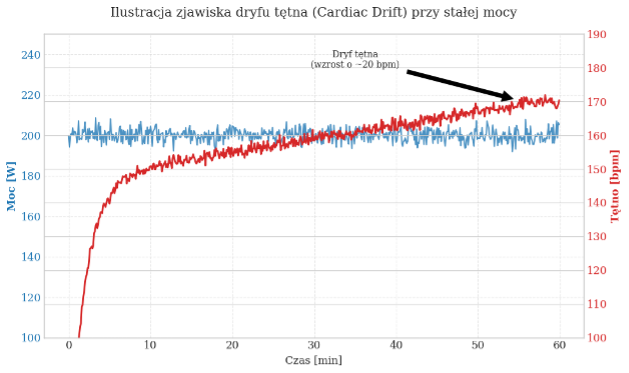
\includegraphics[width=0.95\linewidth]{figures/fig1_hr_drift_hr_lag.png}
  \caption{Ilustracja zjawiska dryfu tętna przy stałej mocy oraz widoczne opóźnienie narastania tętna (\textit{HR lag}) w początkowej fazie wysiłku \cite{nomadfrontiers_power_hr,bikeradar_power_hr}. Źródło: Opracowanie własne.
  }
  \label{fig:hr_drift_hr_lag}
\end{figure}

Dodatkowo:
\begin{itemize}
  \item \textbf{Zmęczenie i wyczerpanie.} Gdy intensywność przekracza zdolność organizmu do stabilnego utrzymania równowagi metabolicznej, narastające zmęczenie prowadzi do konieczności zmniejszenia mocy. W testach $\mathrm{FTP}$ objawia się to przerwaniem wysiłku lub znaczącym obniżeniem mocy, co widać jako spadek mocy na wykresie \cite{borszcz2018ftp,karsten2021cpftp}.
\end{itemize}

Z perspektywy modelu uczenia maszynowego oznacza to, że:
\begin{itemize}
  \item sygnał tętna zawiera informację o reakcji organizmu na obciążenie (moc),
  \item relacja moc--tętno jest nieliniowa i zmienia się w czasie (dryf, narastające zmęczenie),
  \item pojedynczy test $\mathrm{FTP}$ jest jedynie pojedynczym pomiarem tej relacji w konkretnych warunkach oraz w konkretnym dniu.
\end{itemize}

Dlatego sensowne jest podejście, w którym model uczy się tej relacji z wielu treningów, zamiast polegać wyłącznie na jednym teście \cite{stockwell2023mlftp,denham2020predictftp}.

\subsection{Test 20-minutowy -- przebieg i ilustracja}

Najpopularniejszy protokół używany w praktyce do wyznaczania $\mathrm{FTP}$ to test $20$-minutowy \cite{allen2019power,sitko2023_ac20to60_update,phasescycling2023_ftp_variability}.
W literaturze i poradnikach trenerskich spotyka się różne wersje, ale typowy schemat wygląda następująco:
\begin{itemize}
  \item \textbf{Rozgrzewka} (ok.\ $10$--$20$ minut): jazda o niskiej i umiarkowanej intensywności, często z krótkimi przyspieszeniami.
  \item \textbf{Wysiłki przygotowujące} (ang.\ \textit{openers}): krótki, kilku-minutowy wysiłek na wysokiej intensywności (np.\ $3$--$5$ minut powyżej $\mathrm{FTP}$), a następnie etap spokojnej jazdy.
  \item \textbf{Odpoczynek / spokojna jazda} (kilka--kilkanaście minut): częściowa regeneracja przy utrzymaniu „rozgrzania”.
  \item \textbf{Część główna}: $20$-minutowy wysiłek maksymalny; zawodnik stara się utrzymać możliwie najwyższą średnią moc przez pełne $20$ minut.
\end{itemize}

\begin{figure}[htbp]
  \centering
  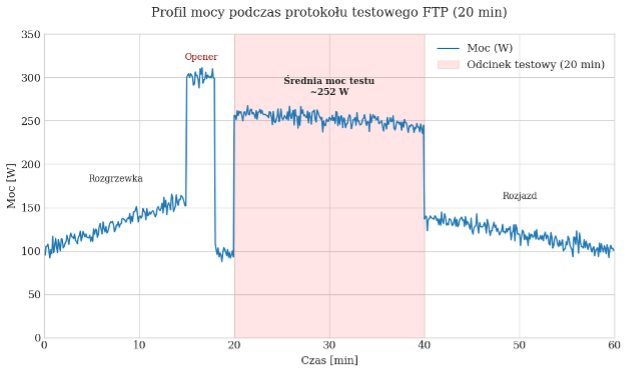
\includegraphics[width=0.95\linewidth]{figures/fig2_ftp_test_20min_schema.png}
  \caption{Schemat przebiegu testu $20$-minutowego $\mathrm{FTP}$: rozgrzewka, wysiłek przygotowujący, okres spokojnej jazdy i $20$-minutowy wysiłek maksymalny. Wynik z otrzymaną średnią należy przemnożyć przez $0{,}95$ \cite{trainerroad_ftp_tips}. Źródło: Opracowanie własne.
  }
  \label{fig:test_20min_schema}
\end{figure}

Dodatkowo można rozważyć drugi wykres, na którym przy stałej mocy podczas $20$-minutowego odcinka widoczny jest stopniowy wzrost tętna jako ilustracja zjawiska dryfu tętna omawianego w poprzedniej sekcji.

\subsection{Test 60-minutowy -- przebieg i ilustracja}

Choć w praktyce trenerskiej najczęściej stosuje się skrócone protokoły (np.\ test $20$-minutowy), pełny, $60$-minutowy test czasowy uznawany jest za najbardziej bezpośrednią i klasyczną metodę wyznaczania $\mathrm{FTP}$.
W ujęciu historycznym $\mathrm{FTP}$ definiowano jako moc, którą zawodnik jest w stanie utrzymać przez pełną godzinę jazdy ciągłej.
Wymaga to jednak bardzo wysokiej dyspozycji, odpowiedniego przygotowania mentalnego oraz sprzyjających warunków, dlatego test stosuje się głównie w środowisku laboratoryjnym lub u doświadczonych kolarzy \cite{allen2019power,sitko2023update}.

Typowy protokół $60$-minutowy można przedstawić następująco:
\begin{itemize}
  \item \textbf{Rozgrzewka} ($15$--$20$ minut): jazda o niższej i umiarkowanej intensywności z kilkoma krótkimi przyspieszeniami.
  \item \textbf{Wstępne pobudzenie} (ang.\ \textit{openers}): kilkuminutowy wysiłek na wysokiej intensywności (np.\ $2$--$4$ minuty powyżej $\mathrm{FTP}$), po którym następuje spokojniejszy fragment jazdy.
  \item \textbf{Krótki etap spokojniejszej jazdy} ($5$--$10$ minut): tętno nieco opada, zawodnik pozostaje przygotowany do części głównej.
  \item \textbf{Część główna}: $60$-minutowy wysiłek submaksymalny o możliwie stałej mocy; średnia moc z tego odcinka jest bezpośrednio interpretowana jako $\mathrm{FTP}$ (bez przelicznika).
\end{itemize}

\begin{figure}[htbp]
  \centering
  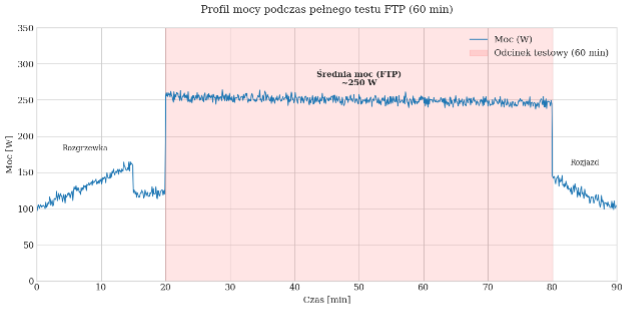
\includegraphics[width=0.95\linewidth]{figures/fig3_ftp_test_60min_schema.png}
  \caption{Schemat przebiegu pełnego testu $60$-minutowego $\mathrm{FTP}$: rozgrzewka, wysiłek przygotowujący, krótki etap spokojnej jazdy oraz główny, godzinny odcinek o możliwie stałej mocy. Średnia moc z $60$-minutowego segmentu stanowi bezpośredni wyznacznik $\mathrm{FTP}$. Źródło: Opracowanie własne.}
  \label{fig:test_60min_schema}
\end{figure}

\subsection{Krzywa mocy i zależność FTP od czasu trwania wysiłku}

Schematyczną zależność maksymalnej możliwej do utrzymania mocy od czasu trwania wysiłku przedstawiono na rysunku \ref{fig:power_duration_curve}.
Dla bardzo krótkich czasów wartości mocy są wysokie i szybko maleją, natomiast przy dłuższych wysiłkach krzywa stopniowo zbliża się do poziomu odpowiadającego mocy krytycznej (ang.\ \textit{Critical Power}, $\mathrm{CP}$), która jest blisko spokrewniona z funkcjonalnym progiem mocy ($\mathrm{FTP}$) \cite{borszcz2018ftp,allen2019power,karsten2021cpftp}.

\begin{figure}[htbp]
  \centering
  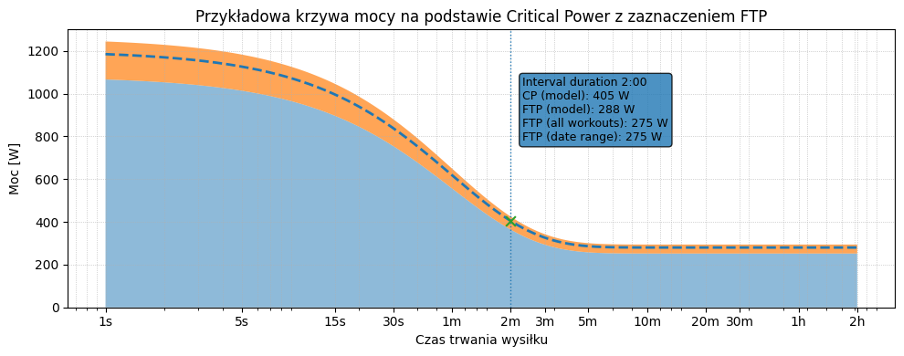
\includegraphics[width=0.95\linewidth]{figures/fig4_power_duration_curve_cp_ftp.png}
  \caption{Przykładowa krzywa mocy (\textit{power--duration}) na podstawie koncepcji mocy krytycznej, z zaznaczonym $2$-minutowym odcinkiem wysiłku i przykładowymi wartościami $\mathrm{FTP}$ (opracowanie własne na podstawie \textit{PerfectPace, The Critical Power Chart}). Źródło: Opracowanie własne.}
  \label{fig:power_duration_curve}
\end{figure}

W praktyce platformy treningowe i oprogramowanie analityczne wykorzystują takie krzywe do estymacji parametrów wydolnościowych, w tym $\mathrm{FTP}$, na podstawie danych z wielu treningów bez konieczności wykonywania osobnego testu \cite{borszcz2018ftp,allen2019power,karsten2021cpftp,denham2020predictftp}.

\section{Charakterystyka danych treningowych}

Modele uczenia maszynowego wykorzystywane do estymacji $\mathrm{FTP}$ opierają się na danych rejestrowanych podczas jazdy na rowerze.
Podstawowym źródłem informacji jest miernik mocy instalowany w korbie, piaście, pedale lub suporcie, który z wysoką częstotliwością (najczęściej $1\ \mathrm{Hz}$) rejestruje chwilową moc generowaną przez kolarza.
Równolegle rejestrowane jest tętno za pomocą opaski na klatkę piersiową lub optycznego czujnika na nadgarstku.
W zależności od konfiguracji sprzętu oraz platformy treningowej możliwe jest także zapisywanie dodatkowych parametrów, takich jak kadencja, prędkość, położenie GPS, nachylenie trasy czy wysokość nad poziomem morza \cite{allen2019power,phases2023ftp,kaggle_cycling_data,figshare_cycling_data}.

W kontekście uczenia maszynowego dane te mają postać szeregów czasowych: dla każdej sekundy otrzymujemy wektor obserwacji zawierający m.in.\ moc [$\mathrm{W}$], tętno [$\mathrm{bpm}$] oraz znacznik czasu.
Dodatkowo dostępne są metadane opisujące daną sesję: typ treningu (jazda spokojna, interwały, wyścig), użyty sprzęt, warunki pogodowe, a także informacja o zawodniku (masa ciała, kategoria wiekowa, poziom sportowy).
Otwarte zbiory danych wykorzystywane w literaturze oraz w niniejszej pracy obejmują zarówno pomiary wykonywane w warunkach laboratoryjnych, jak i dane z rzeczywistych treningów terenowych zapisane w formatach $\mathrm{GPX}$, $\mathrm{FIT}$ czy $\mathrm{CSV}$ \cite{kaggle_cycling_data,figshare_cycling_data,stockwell2023mlftp}.

Kluczową relacją wykorzystywaną przez model jest zależność pomiędzy mocą a tętnem.
Moc odzwierciedla rzeczywistą pracę mechaniczną wykonywaną przez kolarza, natomiast tętno jest miarą reakcji układu krążenia na obciążenie wysiłkiem.
Zależność ta ma charakter nieliniowy i jest modulowana wieloma czynnikami, takimi jak temperatura, poziom odwodnienia, stan zmęczenia czy stosowane leki.
Dodatkowo w trakcie dłuższych wysiłków obserwuje się zjawisko dryfu tętna: stopniowego wzrostu częstości skurczów serca pomimo utrzymywania z grubsza stałej mocy \cite{borszcz2018ftp,karsten2021cpftp}.
Zjawiska te sprawiają, że proste modele liniowe mogą okazać się niewystarczające, natomiast stanowią naturalne pole zastosowania metod uczenia maszynowego zdolnych do modelowania złożonych, nieliniowych zależności \cite{stockwell2023mlftp,denham2020predictftp}.

Istotnym wyzwaniem jest jakość danych treningowych.
W realnych warunkach jazdy rejestrowane szeregi zawierają liczne fragmenty, które nie są bezpośrednio związane z wydolnością tlenową: zjazdy przy niskiej mocy, postoje na skrzyżowaniach, zakłócenia wynikające z utraty sygnału GPS lub błędów odczytu czujników.
Dodatkowo w otwartych zbiorach danych spotyka się brakujące wartości, niespójne nazewnictwo treningów oraz różne częstotliwości próbkowania.
Zanim dane zostaną wykorzystane w modelu, konieczne jest przeprowadzenie operacji wstępnego przetwarzania (filtrowanie, ujednolicanie częstotliwości próbkowania, uzupełnianie lub usuwanie braków oraz segmentacja jazd).

W kolejnych rozdziałach pracy opisane zostaną konkretne zbiory danych użyte w części eksperymentalnej oraz przyjęte decyzje dotyczące ich czyszczenia, łączenia i przygotowania do uczenia modeli.

\section{Klasyczne podejścia a uczenie maszynowe w szacowaniu FTP}

Tradycyjnie do wyznaczania $\mathrm{FTP}$ stosuje się metody oparte na prostych zależnościach matematycznych i z góry ustalonych protokołach testowych.
Przykładem jest $20$-minutowy test czasowy, w którym $\mathrm{FTP}$ definiuje się jako stały procent średniej mocy z próby \cite{allen2019power,sitko2023_ac20to60_update,phasescycling2023_ftp_variability}.
Inne podejścia bazują na modelu mocy--czasu (ang.\ \textit{critical power}, $\mathrm{CP}$), gdzie na podstawie kilku testów o różnym czasie trwania estymuje się parametry krzywej opisującej zależność pomiędzy czasem wysiłku a możliwą do utrzymania mocą \cite{denham2020predictftp}.
W praktyce trenerskiej szeroko wykorzystuje się także progi wyznaczane na podstawie stężenia mleczanu lub wentylacji oddechowej, jednak wymagają one specjalistycznej aparatury laboratoryjnej \cite{borszcz2018ftp,karsten2021cpftp}.

Zaletą klasycznych metod jest prostota i łatwość interpretacji.
Jednocześnie podejścia te zakładają wykonanie jednego lub kilku wysiłków maksymalnych w kontrolowanych warunkach, a uzyskana wartość ma charakter punktowy (opisuje stan zawodnika w chwili testu).
Zmiany wydolności pomiędzy testami pozostają niewidoczne, co utrudnia bieżące monitorowanie adaptacji treningowych \cite{denham2020predictftp,phasescycling2023_ftp_variability}.

Rozwój uczenia maszynowego oraz dostęp do dużych zbiorów danych treningowych otwierają alternatywną ścieżkę: zamiast opierać się wyłącznie na dedykowanych testach, można wykorzystać informacje zawarte w codziennych jazdach.
W literaturze pojawiają się projekty open-source, w których na podstawie historii treningów buduje się modele regresyjne przewidujące wartość $\mathrm{FTP}$ wyznaczoną testem referencyjnym \cite{stockwell2023mlftp,denham2020predictftp}.
Rozwiązania te stanowią naturalny punkt odniesienia (\textit{baseline}) dla niniejszej pracy i pokazują, że podejście oparte na danych ma potencjał praktycznego zastosowania.

Typowo stosowane modele można podzielić na dwie główne grupy:
\begin{itemize}
  \item \textbf{Modele oparte na cechach zagregowanych.} Z surowych szeregów czasowych wyznacza się zestaw cech opisujących jazdę lub jej fragment (np.\ średnia moc i tętno, maksymalna moc z $5$- czy $20$-minutowego okresu, czas w strefach, miary zmienności). Na tak przygotowanych danych uczone są algorytmy regresji, takie jak regresja liniowa, lasy losowe (\textit{Random Forest}) czy modele \textit{gradient boosting} (np.\ \textit{XGBoost}). Zaletą jest interpretowalność i relatywnie niewielkie wymagania obliczeniowe \cite{stockwell2023mlftp}.
  \item \textbf{Modele sekwencyjne.} Podejście polega na bezpośrednim modelowaniu szeregów czasowych (bez redukcji do kilku wskaźników). Wykorzystuje się architektury neuronowe takie jak $\mathrm{LSTM}$, $\mathrm{GRU}$ czy modele typu \textit{Transformer} przystosowane do danych czasowych. Umożliwia to uchwycenie złożonych wzorców dynamiki wysiłku, jednak wymaga większej ilości danych, starannego doboru hiperparametrów i jest trudniejsze do interpretacji \cite{stockwell2023mlftp}.
\end{itemize}

Oba podejścia nie wykluczają się wzajemnie.
W praktyce często tworzy się hybrydowe pipeline'y, w których część informacji pochodzi z cech zagregowanych, a część z modeli sekwencyjnych.
W niniejszej pracy przyjęto podejście regresyjne, w którym $\mathrm{FTP}$ traktowane jest jako zmienna ciągła, a celem jest minimalizacja błędu predykcji względem wartości referencyjnych wyznaczonych testami.

\subsection{Przegląd algorytmów regresyjnych w analizie danych sportowych}

Wybór algorytmu do estymacji parametrów fizjologicznych jest kluczowy dla skuteczności modelu.
W literaturze przedmiotu najczęściej wymienia się następujące podejścia \cite{stockwell2023mlftp}:

\subsubsection{Modele liniowe i regularyzacja}

Podstawowym narzędziem w zadaniach predykcji wartości ciągłej (jaką jest $\mathrm{FTP}$) jest regresja liniowa.
Zakłada ona liniową zależność między cechami wejściowymi (np.\ średnim tętnem, mocą z określonych przedziałów czasowych) a zmienną celu.
Choć fizjologia wysiłku ma charakter nieliniowy, modele liniowe stanowią dobry punkt odniesienia (\textit{baseline}).
Aby zapobiec przeuczeniu przy dużej liczbie skorelowanych cech, stosuje się regularyzację:
\begin{itemize}
  \item \textbf{Lasso} ($\ell_1$) - umożliwia selekcję cech poprzez zerowanie współczynników przy mniej istotnych zmiennych,
  \item \textbf{Ridge} ($\ell_2$) - zmniejsza wariancję modelu, co jest korzystne przy współliniowości danych treningowych.
\end{itemize}

\subsubsection{Metody zespołowe (ang.\ \textit{Ensemble Learning})}

Jednymi z najskuteczniejszych algorytmów w pracy z danymi tabelarycznymi są metody oparte na drzewach decyzyjnych.
Pojedyncze drzewo ma tendencję do nadmiernego dopasowania, dlatego stosuje się:
\begin{itemize}
  \item \textbf{\textit{Random Forest}} - wykorzystuje bagging (\textit{bootstrap aggregating}); trenuje wiele drzew na losowych podzbiorach danych i uśrednia ich wyniki.
  \item \textbf{\textit{Gradient Boosting}} (np.\ \textit{XGBoost}, \textit{LightGBM}, \textit{CatBoost}) - buduje model sekwencyjnie, gdzie kolejne drzewa korygują błędy poprzednich.
\end{itemize}

\subsubsection{Sieci neuronowe i głębokie uczenie (ang.\ \textit{Deep Learning})}

Gdy dane wejściowe traktujemy jako surowy szereg czasowy (sekwencja próbek moc/tętno co $1$ sekundę), intensywna inżynieria cech może prowadzić do utraty informacji o dynamice zmian.
W takich przypadkach zastosowanie znajdują:
\begin{itemize}
  \item rekurencyjne sieci neuronowe ($\mathrm{RNN}$) oraz $\mathrm{LSTM}$,
  \item konwolucyjne sieci neuronowe $1\mathrm{D}$ ($1\mathrm{D}$-$\mathrm{CNN}$),
  \item modele typu \textit{Transformer} dla szeregów czasowych.
\end{itemize}

\section{Zarys procesu przetwarzania danych i budowy modelu}

Zastosowanie uczenia maszynowego do estymacji $\mathrm{FTP}$ wymaga zdefiniowania spójnego procesu przetwarzania danych obejmującego następujące etapy.

\paragraph{Pozyskanie i integracja danych.}
W pracy wykorzystane zostaną otwarte zbiory danych zawierające zarówno wyniki testów wydolnościowych, jak i towarzyszące im szeregi czasowe mocy oraz tętna \cite{kaggle_redlineracer_road_cycling_performance_testing,figshare_cycling_analytics_datasets,stockwell2023mlftp}.
Dodatkowo rozważona może zostać integracja z innymi źródłami (np.\ pliki $\mathrm{GPX}/\mathrm{FIT}$ z regularnych jazd terenowych).

\paragraph{Wstępne przetwarzanie danych.}
Obejmuje ono m.in.\ filtrację artefaktów pomiarowych, ujednolicenie częstotliwości próbkowania oraz obsługę brakujących wartości.
Jakość tego etapu ma bezpośredni wpływ na stabilność cech i modeli.

\paragraph{Definicja etykiet.}
Naturalnym wyborem jest $\mathrm{FTP}$ wyznaczone na podstawie standaryzowanego testu referencyjnego (np.\ testu $20$-minutowego skorygowanego współczynnikiem) lub wyniku laboratoryjnego odpowiadającego mocy progowej \cite{borszcz2018ftp,karsten2021cpftp,denham2020predictftp}.
Następnie dla treningów wykonywanych w określonym oknie czasowym względem testu (np.\ $\pm 2$ tygodnie) przyjmuje się tę samą wartość $\mathrm{FTP}$, co pozwala przypisać etykietę do wielu sesji bez wykonywania dodatkowych testów \cite{stockwell2023mlftp,denham2020predictftp}.
Jest to świadome założenie modelowe: w krótkim horyzoncie czasu $\mathrm{FTP}$ zmienia się relatywnie wolno.

\paragraph{Inżynieria cech.}
Z surowych danych wyznacza się cechy opisujące wysiłek i reakcję organizmu: średnie i maksymalne moce w oknach czasowych, rozkład czasu w strefach, relacje moc--tętno (\textit{power-to-heart-rate ratio}), miary zmienności tętna oraz wskaźniki dryfu tętna.

\paragraph{Trening i ewaluacja.}
Zbiór danych dzielony jest na część treningową, walidacyjną i testową z uwzględnieniem unikania wycieku informacji (\textit{data leakage}), np.\ poprzez grupowanie obserwacji na poziomie zawodnika lub bloku czasowego.
Do strojenia hiperparametrów stosuje się walidację krzyżową lub podział czasowy.
Jako miary jakości predykcji stosuje się typowo $\mathrm{MAE}$, $\mathrm{RMSE}$ oraz miary korelacji i determinacji, w tym $R^2$ \cite{james2021isl,hastie2009esl}.

\subsection{Metryki ewaluacji modelu}

Aby obiektywnie ocenić jakość estymacji $\mathrm{FTP}$ przez model, konieczne jest zdefiniowanie miar błędu.
W problemach regresji standardowo stosuje się m.in.\ następujące metryki \cite{james2021isl,hastie2009esl}.

\paragraph{Pierwiastek błędu średniokwadratowego (RMSE).}
\begin{equation}
\label{eq:rmse}
\mathrm{RMSE} = \sqrt{\frac{1}{n}\sum_{i=1}^{n}\left(y_i - \hat{y}_i\right)^2},
\end{equation}
gdzie $y_i$ oznacza rzeczywistą wartość $\mathrm{FTP}$ (wyznaczoną na podstawie testu referencyjnego), a $\hat{y}_i$ odpowiadającą jej wartość przewidywaną przez model.
$\mathrm{RMSE}$ jest wrażliwy na duże błędy (obserwacje odstające), co jest pożądane w zastosowaniach sportowych, ponieważ duże pomyłki mogłyby prowadzić do niewłaściwego doboru obciążeń treningowych.

\paragraph{Średni błąd bezwzględny (MAE).}
\begin{equation}
\label{eq:mae}
\mathrm{MAE} = \frac{1}{n}\sum_{i=1}^{n}\left|y_i - \hat{y}_i\right|.
\end{equation}
$\mathrm{MAE}$ jest łatwiejsze w interpretacji dla trenera, ponieważ wprost mówi, o ile watów średnio myli się model (np.\ „średni błąd wynosi $5\ \mathrm{W}$”).

\paragraph{Współczynnik determinacji ($R^2$).}
\begin{equation}
\label{eq:r2}
R^2 = 1 - \frac{\sum_{i=1}^{n}\left(y_i - \hat{y}_i\right)^2}{\sum_{i=1}^{n}\left(y_i - \bar{y}\right)^2},
\end{equation}
gdzie $\bar{y}$ oznacza średnią wartość rzeczywistego $\mathrm{FTP}$ w próbie.
Wartość bliska $R^2 = 1$ oznacza bardzo dobre dopasowanie modelu do danych, natomiast wartości ujemne świadczą o tym, że model przewiduje gorzej niż proste przyjęcie średniej z próby.
W badaniach nad wydolnością wysokie wartości $R^2$ (np.\ powyżej $0{,}9$) pomiędzy wynikami testów skróconych a pełnymi bywają interpretowane jako przesłanka użyteczności danej metody estymacji \cite{karsten2021cpftp}.